% !TEX root = main.tex

\section{Analysis}

The following analysis will be presented in two parts, one which will be before filtering with timedomain response of the two signals and then the frequency analysis of these with poles and zeroes. Next an appropriate filter will be applied and the two signals will again be analysed as previously explained.

\subsection{Before filtering}

\subsubsection{Timedomain analysis}

Firstly an formal analysis of the man and the womans voice saying "Hej Lasse" in the timedomain. In \cref{fig:time_man} the signal for the man can be seen, with the time in seconds on the x-axis and the magnitude on the y-axis and similarily the womans signal is shown in \cref{fig:time_woman}.

\begin{figure}
\centering
\begin{subfigure}{0.45\textwidth}
	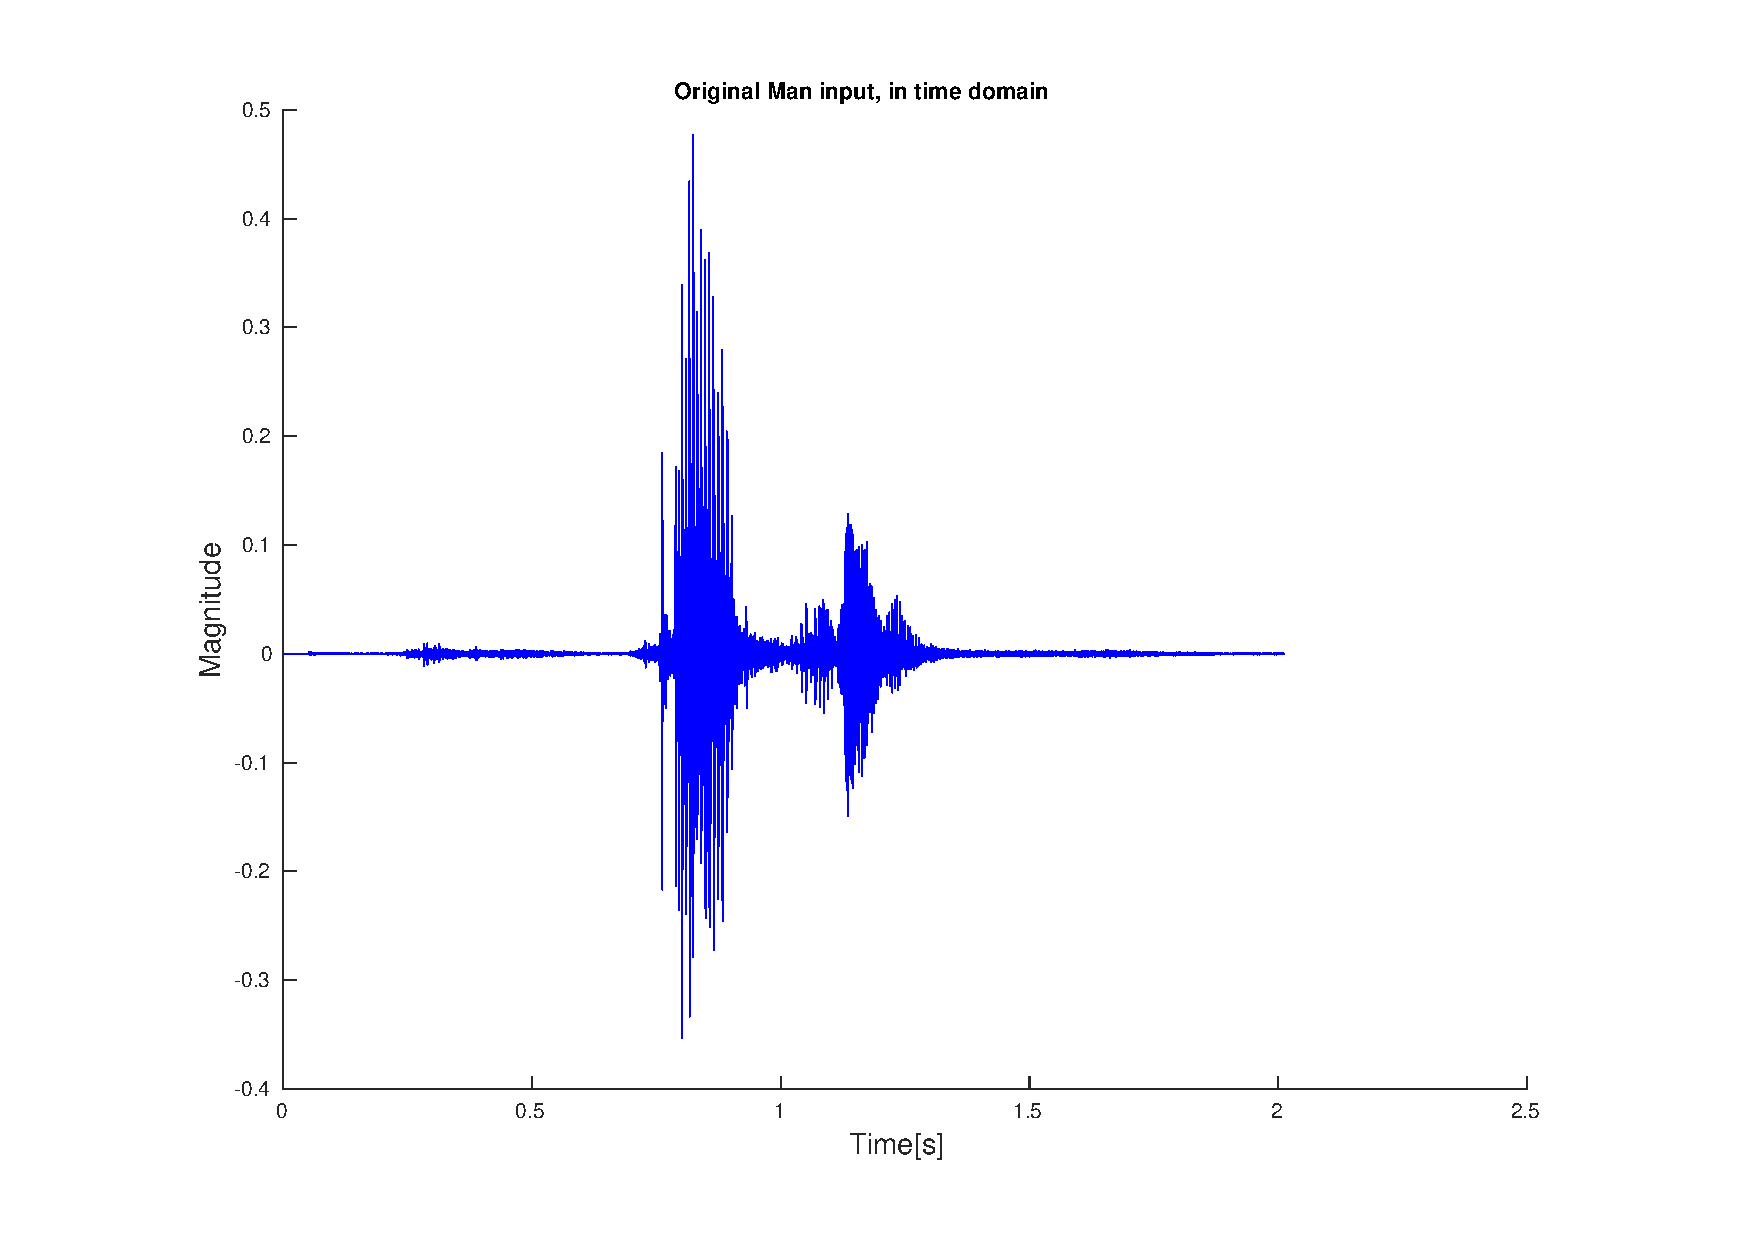
\includegraphics[width=\textwidth]{OrgTid_Man.pdf}
	\caption{The time domain signal of the man}
	\label{fig:time_man}
\end{subfigure}
\quad
\begin{subfigure}{0.45\textwidth}
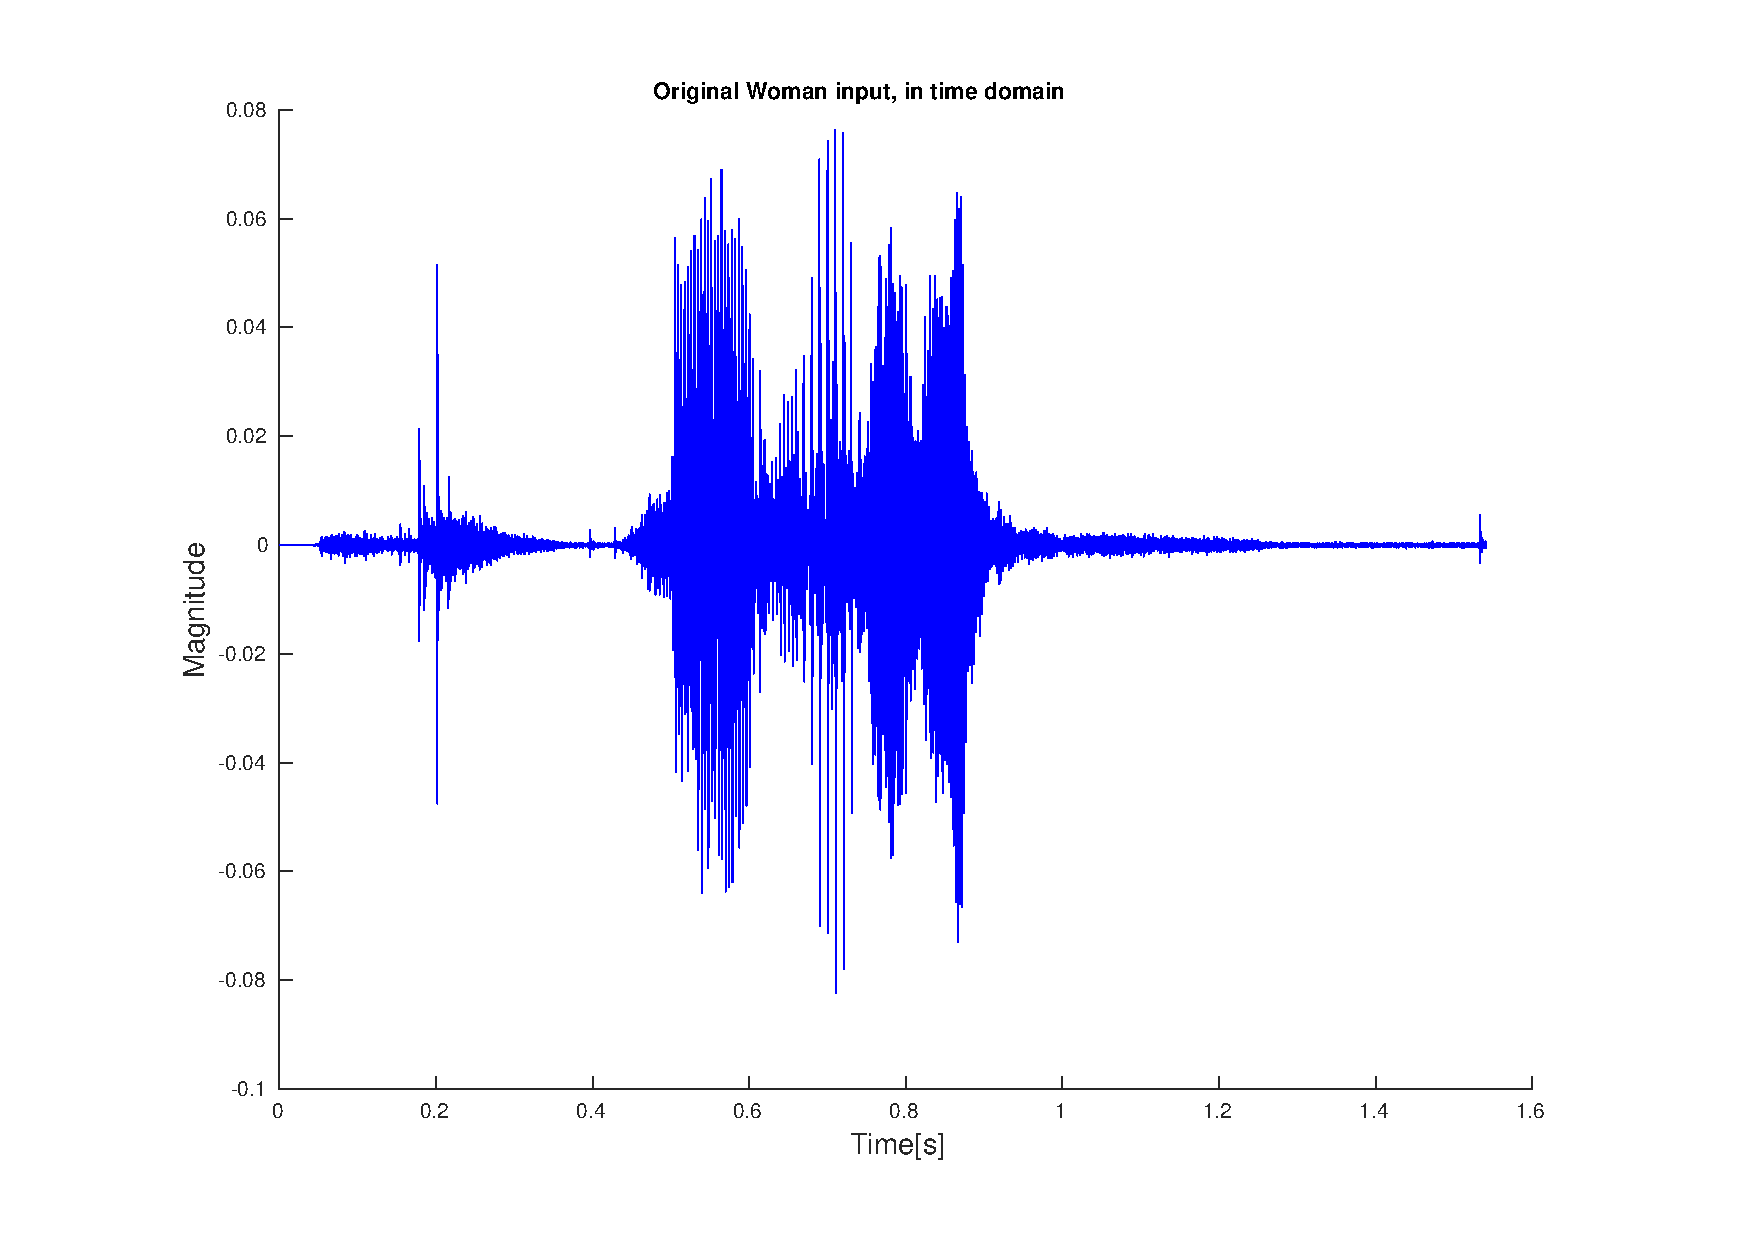
\includegraphics[width=\textwidth]{OrgTid_Woman.pdf}
\caption{The time domain signal of the woman}
\label{fig:time_woman}
\end{subfigure}
\caption{The timesamples of a man and a woman saying "Hej Lasse"}
\label{fig:time_WoMan}
\end{figure}

\subsubsection{Fourier transform with FFT}

The fourier transform will show the characteristics of the male and female voice. In \cref{fig:WoManFFT} the fourier transform based of the two privious signals seen in \cref{fig:time_WoMan} - in red the male signal and in blue the female signal.

\begin{figure}
\centering
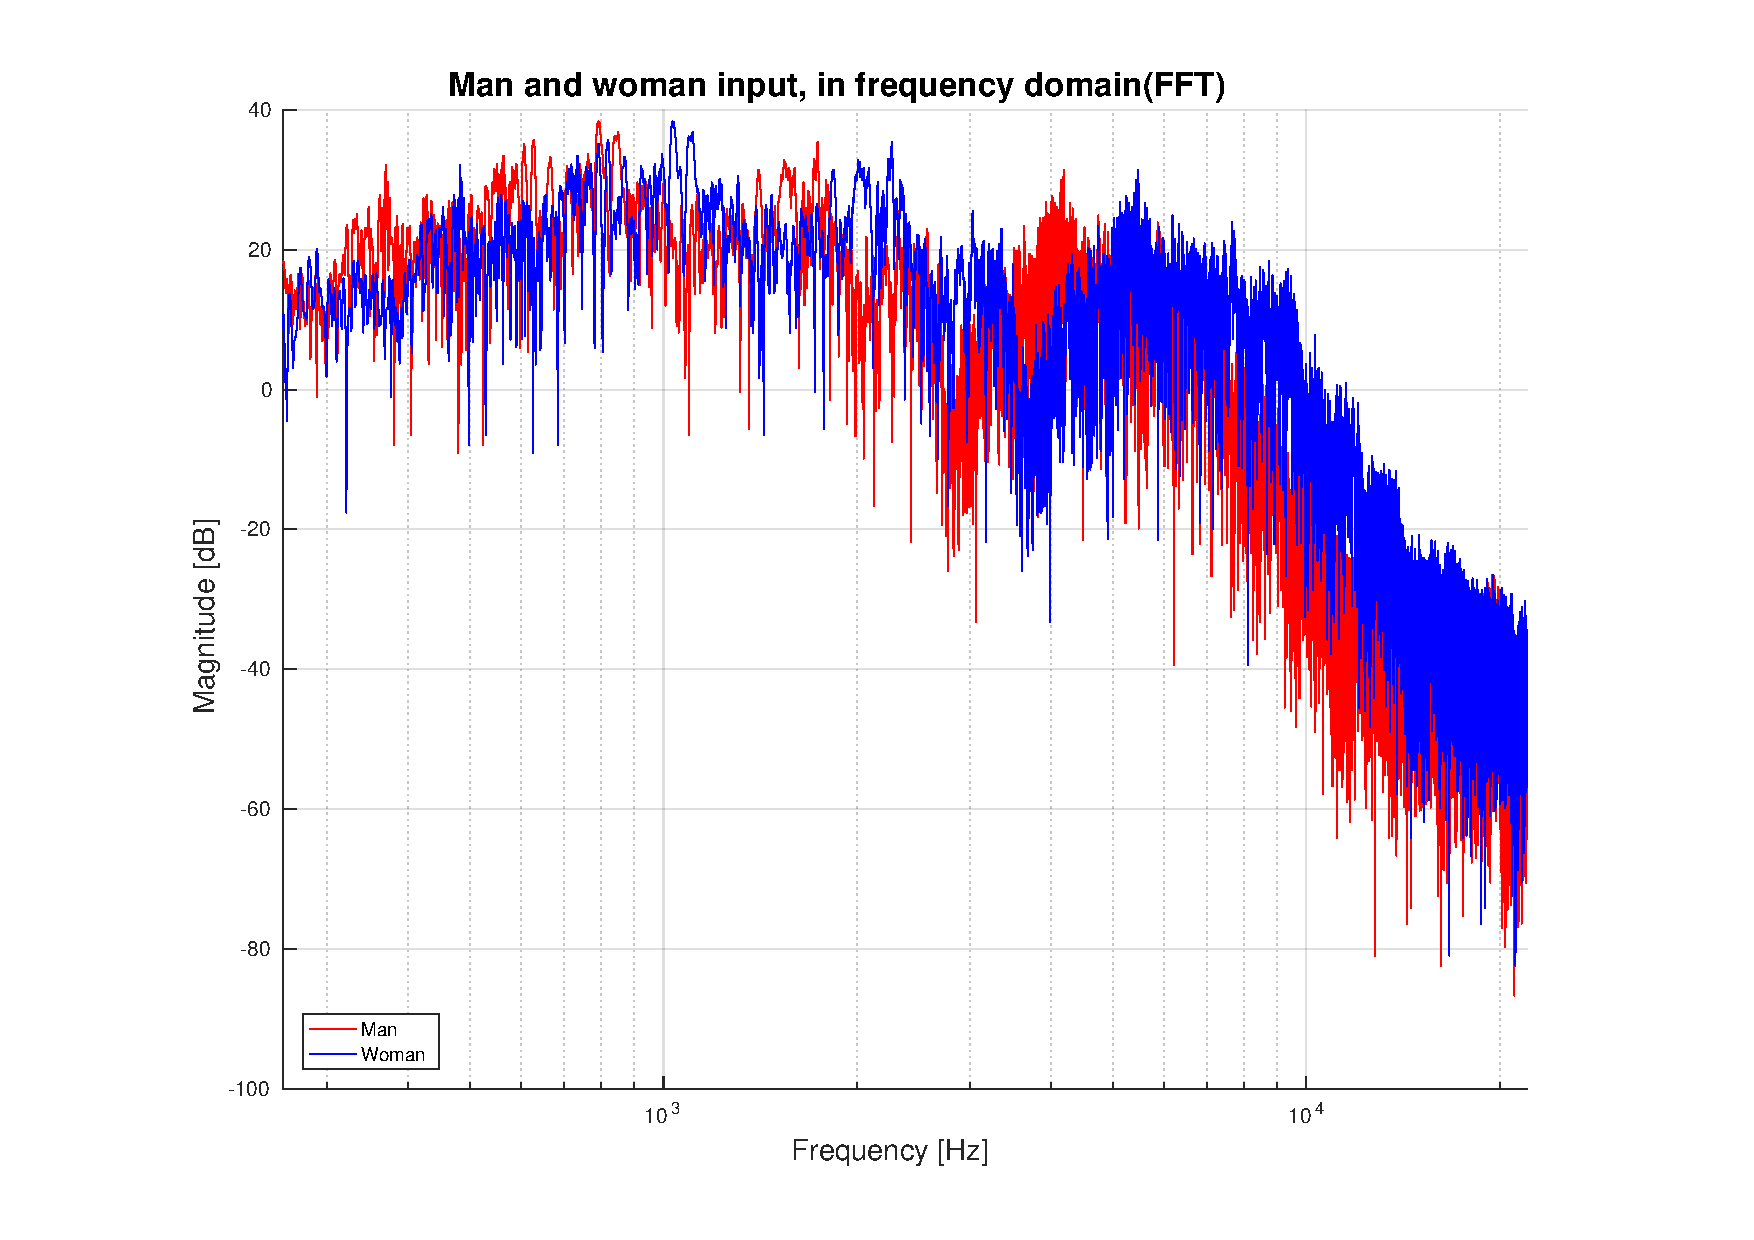
\includegraphics[width=\textwidth]{OrgFreq_WoMan.pdf}
\caption{The frequency analysis of the man and woman}
\label{fig:WoManFFT}
\end{figure}

\subsection{Filtering}

